\chapter{Implementación}
\label{cap6}

El desarrollo de la aplicación se ha dividido en diferentes etapas que se explicarán a continuación, según el lenguaje y la funcionalidad que se estaba implementando en cada momento. Todo el código está disponible en \href{https://github.com/nazaretrogue/Android-Shield}{\textcolor{blue}{github.com/nazaretrogue/Android-Shield}}.

\section{Implementación de la aplicación en Java}

La aplicación en sí se implementó en Java por varias razones:

\begin{itemize}
	\item Es el lenguaje oficial de Android. Aunque hay muchas aplicaciones hechas en Kotlin, no está oficialmente respaldado por Google.
	\item Java es un lenguaje orientado a objetos.
	\item Tiene muchas bibliotecas, frameworks y una extensa documentación, lo que facilita la programación y abstrae al programador al llevar a cabo casi cualquier tarea.
	\item El tiempo de ejecución de una aplicación en Java es menor que una aplicación en Kotlin. Además, el tamaño de la biblioteca estándar de Kotlin es mayor, lo que hará que la aplicación pese más que si se hace en Java.
\end{itemize}

La creación de la tarea principal de la aplicación se llevó a cabo en diferentes etapas, empezando por la implementación de la interfaz de usuario. La apariencia de la aplicación es sencilla: una pantalla negra en forma de consola que contiene un cuadro desplazable de texto en el que se escribe en blanco el resultado del análisis. Para activar el análisis de las aplicaciones instaladas hay un botón flotante que inicia el modelo de Python para predecir la clasificación de cada una.

Una vez que la interfaz de usuario estaba construida, se procedió a implementar la actividad en sí. Para ello, se necesitaba un listado de las aplicaciones del dispositivo, así que se utilizó el contexto. El contexto de una aplicación en Android contiene información sobre el entorno en el que la actividad de la app se está desarrollando. A través de él se puede acceder a información del dispositivo como, por ejemplo, el estado actual de la aplicacion en sí, las actividades que se están llevando a cabo en segundo plano o la lista de aplicaciones instaladas en el dispositivo, ente otros.

Se crearon dos clases para modularizar la aplicación:

\begin{enumerate}
	\item \textbf{Clase \textit{Permisos}}: contiene un array con los permisos peligrosos en forma de cadena de cada aplicación y un map con dichos permisos en binario. Hay diferentes métodos para trabajar fácilmente con esta información y abstraerla de la actividad principal.
	\item \textbf{Clase \textit{Aplicacion}}: contiene el nombre y los permisos de cada aplicación. Constituye una unidad sencilla que almacena la información y las operaciones que necesita el detector de malware.
\end{enumerate}

Tras tener las clases implementadas, se procedió a implementar la actividad principal. Ésta utiliza el contexto del detector y extrae todos los permisos de las aplicaciones, que después son filtrados para quedarse solo con los permisos peligrosos. También extrae el nombre de la aplicación para crear un objeto \textit{Aplicacion} que se envía al modelo para que prediga la clasificación.

\section{Implementación de scripts en Python}

A la hora de implementar el modelo a entrenar, las opciones al elegir lenguaje eran mucho más amplias que para hacer la actividad principal, pero se eligió Python por varios motivos:

\begin{itemize}
	\item Es un lenguaje sencillo de entender e implementar.
	\item Hay muchas bibliotecas para desarrollar proyectos de \textit{Machine Learning}, con muchos algoritmos distintos, funcionalidades y herramientas variadas que facilitan la implementación.
	\item Es uno de los  lenguajes con mejor rendimiento a la hora de ejecutar programas que implican \textit{Machine Learning}.
	\item La integración con otros lenguajes es relativamente sencilla.
\end{itemize}

Una vez creada la aplicación, se implementó la parte de Python. A pesar de que no es la actividad principal como tal pues la mayor parte del código no se ejecuta en la app sino antes, esta fase es el grueso de este trabajo.

\subsection{Preprocesador de aplicaciones de muestra}

El primer paso fue implementar un preprocesador para las muestras. El script recibe el \textit{path} en el que están almacenadas las muestras y extrae los permisos de cada aplicación para almacenarlos en un archivo junto con la etiqueta de dicha app.

Se utilizaron un total de 34549 muestras: 14799 aplicaciones malignas y 19750 aplicaciones benignas. Las aplicaciones benignas se extrajeron de la \textit{Play Store}, mientras que las muestras de malware fueron extraídas de distintas bases de datos (Tabla~\ref{tab:dataset}). El archivo con las aplicaciones preprocesadas contiene 31 columnas correspondientes a los 30 permisos peligrosos y a la etiqueta de la aplicación. Los permisos están ordenados por orden alfabético y pueden verse en \textit{\nameref{lista_permisos}}.

\begin{table}[H]
\begin{tabular}{|c|c|c|c|c|}
\hline
\textbf{Nombre} & \textbf{Tipo} & \textbf{Fecha} & \textbf{Nº de muestras} & \textbf{Referencia} \\ \hline
AMD Project     & Malware       & 2018-2019      & 5500                    & \hypersetup{citecolor=red}\cite{amd}                    \\ \hline
Google Play     & Benigna       & 2021           & 19750                   & \hypersetup{citecolor=red}\cite{playstore}                    \\ \hline
VirusShare      & Malware       & 2018-2019      & 8299                    & \hypersetup{citecolor=red}\cite{virusshare}                    \\ \hline
VirusTotal      & Malware       & 2018-2020      & 1000                    & \hypersetup{citecolor=red}\cite{virustotal}                    \\ \hline
\end{tabular}
\caption{Datasets de aplicaciones}
\label{tab:dataset}
\end{table}

\subsection{Script de entrenamiento}

Una vez que las aplicaciones estaban preprocesadas, ya se podía implementar el modelo. Utilizando la biblioteca Scikit Learn, al principio opté por un \textit{Naives Bayes Classifier} (o \textit{Clasificador Bayesiano Ingenuo}), en el que cada característica o \textit{feature} (en este caso cada permiso) es independiente del resto. El algoritmo clasificaba, por tanto, cada aplicación según los permisos que utilizaba sin tener en cuenta la relación entre ellos; por ejemplo, si la mayoría de malware que solicita permiso de lectura de los contactos también solicita permiso de escritura de mensajes SMS, el clasificador ingenuo desecharía dicha relación.

De todas las muestras recogidas, el 80\% de éstas (elegidas aleatoriamente) se utilizó para entrenar al modelo y el 20\% restante se usó para hacer los tests.

Tras entrenar al modelo, la \textit{accuracy} o precisión era de solo un 79\%; para incrementar la precisión, se llevó a cabo un PCA (análisis de componentes principales), una técnica que analiza cada \textit{feature} y elimina aquellas que no son útiles para diferenciar entre aplicación benigna o malware. Es decir, lo que hace la técnica del PCA es eliminar el ruido introducido por las \textit{features} que lo único que hace es ``confundir'' al clasificador. Desgraciadamente, la precisión solo se incrementó hasta alcanzar un 84\%. Para ver mejor el resultado, se generó una curva ROC (Figura~\ref{fig:roc1}), una representación gráfica que muestra la precisión del clasificador.

\begin{figure}[H]
\centering
	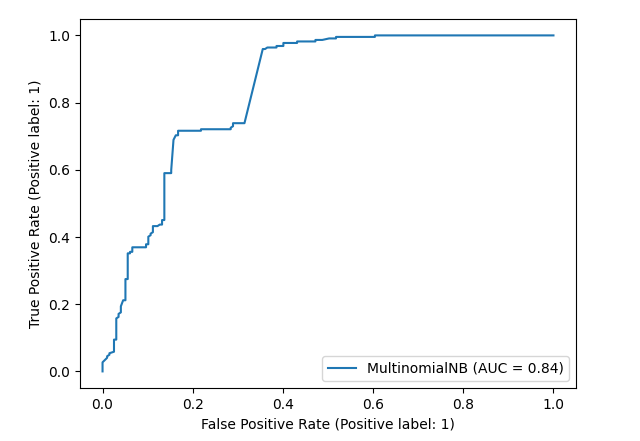
\includegraphics[scale=0.6]{img/roc-84.png}
	\caption{Curva ROC con el clasificador bayesiano}
	\label{fig:roc1}
\end{figure}

Puesto que el resultado no era el esperado, hubo que cambiar de algoritmo. Según el problema al que nos enfrentamos, la selección del algoritmo es fundamental si queremos obtener resultados prometedores\hypersetup{citecolor=red}\cite{oreilly}. Debido a la naturaleza de los datos del problema, el número de \textit{features} (permisos) y el propósito del análisis (la clasificación de aplicaciones), se decidió utilizar un algoritmo algo más complejo y sofisticado como la \textit{Support Vector Machine} o SVM (\textit{Máquina de Vector Soporte}), más apropiado para tratar con el problema de diferenciar entre aplicaciones benignas o malware. Aunque el clasificador bayesiano puede ser efectivo en otros problemas de clasificación, en este en concreto no lo es, pues ignora la relación que puede haber entre dos \textit{features}, lo que se traduce en un decremento de la precisión. SVM no ignora la relación entre \textit{features}, así que la precisión obtenida mejora notablemente.

El SVM es un clasificador capaz de distinguir, en un espacio finito de muestras, entre dos subconjuntos, en este caso entre que la aplicación sea benigna o maligna. El SVM busca un hiperplano para separar ambos subconjuntos según las dimensiones del espacio en el que se encuentran las muestras. Por ejemplo, en un espacio 2D, el SVM buscará una recta que separe ambos subconjuntos y que permita la mayor distancia entre ellos.

Después de hacer los tests, el clasificador SVM junto con la técnica del PCA dio una precisión del 99\%. Se utilizó también \textit{cross-validation}, una técnica que permite comprobar el \textit{overfitting} o sobreajuste del modelo a los datos de entrenamiento.

El resultado, por tanto, era satisfactorio.

\begin{figure}[H]
\centering
	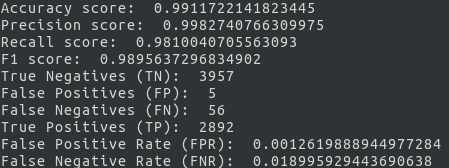
\includegraphics[scale=0.8]{img/accuracy.png}
	\caption{Precisión del modelo entrenado}
\end{figure}

\begin{figure}[H]
\centering
	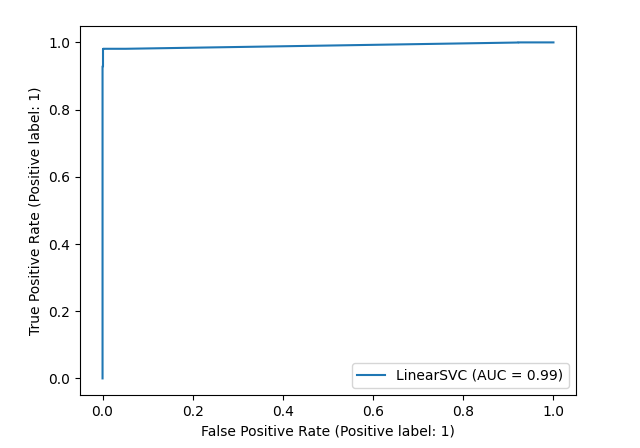
\includegraphics[scale=0.6]{img/roc.png}
	\caption{Curva ROC con el clasificador SVM}
\end{figure}

Una vez obtenidos los resultados deseados, tanto el modelo PCA como el modelo SVM se guardaron en sendos archivos binarios mediante la biblioteca \textit{Pickle} para después poder utilizarlos en el script de predicción.

En la Tabla~\ref{tab:metricas} podemos ver los resultados obtenidos por \textit{Android Shield}:

\begin{itemize}
	\item FPR (\textit{False Positive Rate}) es el porcentaje de falsos positivos, es decir, el número de aplicaciones clasificadas como malware cuando en realidad son aplicaciones benignas.
	\item FNR (\textit{False Negative Rate}) es el porcentaje de falsos negativos, o sea, el número de aplicaciones erróneamente clasificadas como aplicaciones benignas cuando en realidad son malware.
	\item TN (\textit{True Negative}) es el número de aplicaciones clasificadas correctamente como aplicaciones benignas de un total de 6910 aplicaciones utilizadas en los tests.
	\item FP (\textit{False Positive}) es el número de aplicaciones clasificadas erróneamente como malware cuando son benignas.
	\item FN (\textit{False Negative}) es el número de aplicaciones clasificadas erróneamente como aplicaciones benignas cuando en realidad son malware.
	\item TP (\textit{True Positive}) es el número de aplicaciones correctamente clasificadas como malware.
\end{itemize}

\begin{table}[H]
\centering
\begin{tabular}{|c|c|}
\hline
\textbf{Métrica} & \textbf{Resultado}  \\ \hline
Accuracy & 99.11\% \\ \hline
FPR & 0.12\% \\ \hline
FNR & 1.89\% \\ \hline
TN & 3957 \\ \hline
FP & 5 \\ \hline
FN & 56 \\ \hline
TP & 2892 \\ \hline
\end{tabular}
\caption{Resultados de \textit{Android Shield}}
\label{tab:metricas}
\end{table}

\subsection{Script de predicción}

Una vez que el modelo estaba entrenado, se implementó el script en el que se predecía si una app dada era o no malware. Dicho script recibe un nombre de aplicación y el array binario con los permisos peligrosos de dicha aplicación.

En este script, tras cargar el modelo del PCA y el del SVM, se filtran los permisos con el PCA para obetener las \textit{features} que realmente se utilizan para clasificar la app, y una vez hecho esto, se predice la app utilizando el modelo entrenado y éste devuelve la etiqueta de la clasificación.

Antes de integrarlo con la aplicación de \textit{Android Shield}, se hicieron pruebas para comprobar el funcionamiento (razón por la cual hay una función \textbf{main} en dicho script a pesar de no ser necesaria para su ejecución en la aplicación).

\section{Integración Java-Python}

Tras haber comprobado el correcto funcionamiento de modelo, se llevó a cabo la integración entre la aplicación y el modelo. Al ser dos lenguajes diferentes, se necesitaba un soporte extra, como \textit{Weka}, \textit{Jython} o \textit{ApacheSpark}. No obstante, se optó por una opción más sencilla pero de la que fue necesario solicitar una licencia Chaquopy; de esta forma, la integración entre ambos lenguajes no requiere de bibliotecas externas o extensas modificaciones de código.

Con la licencia activada, solo hubo que modificar ligeramente la actividad principal de la aplicación. Durante la creación de la app se tenía que iniciar Python; una vez hecho esto, se debía crear una instancia de Python desde la cual se llamaría al script de predicción con los parámetros solicitados, es decir, el nombre de la app que se está analizando en cada momento y un array con los permisos peligrosos. 

\section{Pruebas}

Una vez que toda la aplicación estaba ensamblada y en funcionamiento con el modelo correctamente entrenado, se hicieron pruebas de funcionamiento. Al abrir la aplicación aparece una pantalla negra, un botón redondo en la esquina inferior derecha y un mensaje en el que se indica que se debe pulsar dicho botón para inciar el análisis de las aplicaciones instaladas.

Una vez pulsado el botón, hay que esperar un par de segundos para que se complete el análisis y se muestren los resultados en pantalla. Cuantas más aplicaciones haya en el dispositivo, más tiempo tardará el análisis. Se muestra en forma de lista en un cuadro de texto desplazable. Tiene el aspecto de la Figura~\ref{fig:prueba}.

Como se puede observar en la Figura~\ref{fig:prueba}, rodeada con un rectángulo de color verde, hay una aplicación señalada como malware: la aplicación de llamadas. La clasificación de esta app es un falso positivo, como es obvio. No obstante, es inevitable que ocurra, ya que la aplicación de llamadas requiere varios permisos considerados peligrosos: acepta llamadas, puede grabar un mensaje de voz para el contestador, responde y hace llamadas, procesa las llamadas salientes, puede leer y escribir en el log de llamadas, leer y escribir contactos y leer y escribir números de teléfono. Esta prueba demuestra que la aplicación funciona bien por lo general pero que hay aplicaciones que, aunque nosotros sabemos que no son malware, \textit{Android Shield} considera maliciosas.

\begin{figure}[H]
\centering
\begin{minipage}{.5\textwidth}
	\centering
	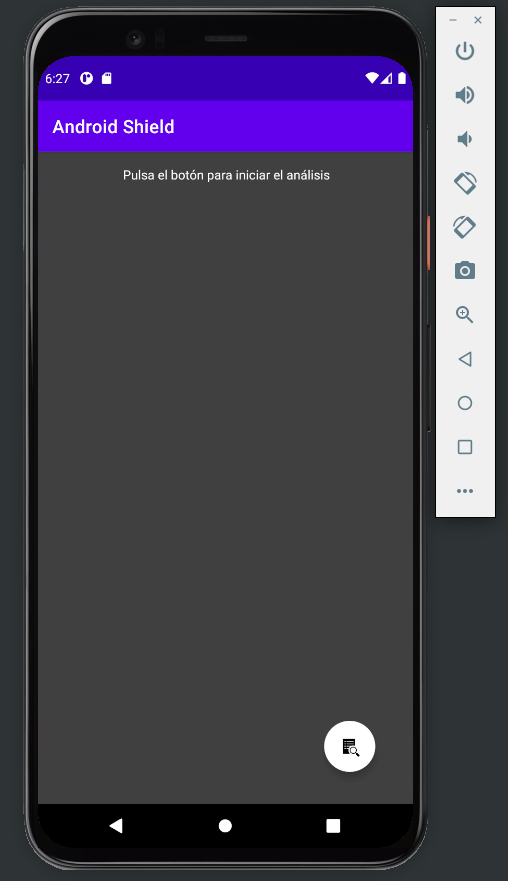
\includegraphics[scale=0.3]{img/emulator.png}
	\captionof{figure}{Pantalla inicial}
	\label{fig:test1}
\end{minipage}%
\begin{minipage}{.5\textwidth}
	\centering
	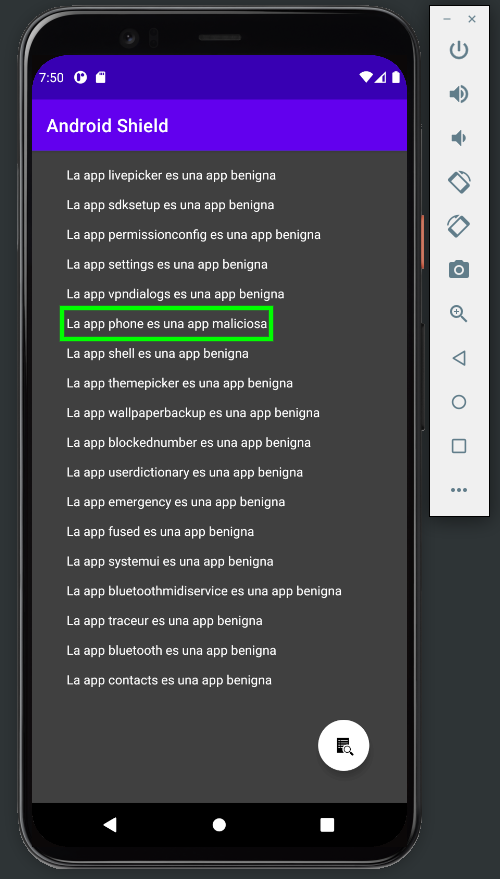
\includegraphics[scale=0.3]{img/test.png}
	\captionof{figure}{Resultado del análisis}
	\label{fig:prueba}
\end{minipage}
\end{figure}

\subsection{Requerimientos del dispositivo}

Ya que el entrenamiento del modelo se lleva a cabo fuera del dispositivo, lo único que hace la actividad principal es cargar dicho modelo para poder analizar las apps instaladas. Eso significa que los costes para ejecutar \textit{Android Shield} son muy bajos y el análisis de malware se lleva a cabo dentro del dispositivo. Esto supone una ventaja frente aquellos detectores de malware que tal vez sean más potentes pero que, debido a los altos requerimientos computacionales, deben llevarse a cabo fuera del dispositivo, como\hypersetup{citecolor=red}\cite{cloud}.

Se han comprobado los requerimientos de CPU, de memoria y de batería de \textit{Android Shield}. La Figura \ref{fig:general} muestra el tiempo de ejecución (alrededor de 4 segundos para analizar 74 aplicaciones, desde el minuto 01:02:00 hasta el 01:06:30 aproximadamente) y el uso de que hace de CPU y memoria durante ese tiempo. También se puede observar que el gasto de batería durante el análisis es mínimo, así que \textit{Android Shield} es una aplicación ligera y que prácticamente no afecta al rendimieto.

\begin{figure}[H]
\centering
	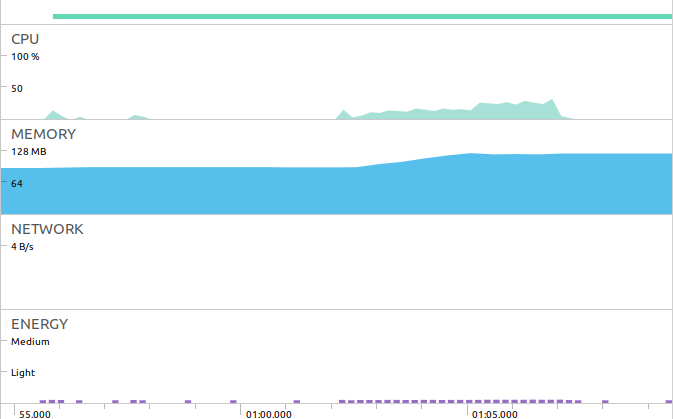
\includegraphics[scale=0.5]{img/general.png}
	\caption{Requerimientos de \textit{Android Shield}}
	\label{fig:general}
\end{figure}

Se ha hecho un zoom en la CPU y en el uso de memoria para que se vea más claramente. En la Figura \ref{fig:memory} además se especifíca para que se está usando la memoria. La mayor parte de la ocupación proviene del propio sistema operativo, aunque cuando se empieza a ejecutar \textit{Android Shield} se muestra un pequeño incremento del uso, que corresponde con la carga del código de Java.

\begin{figure}[H]
\centering
	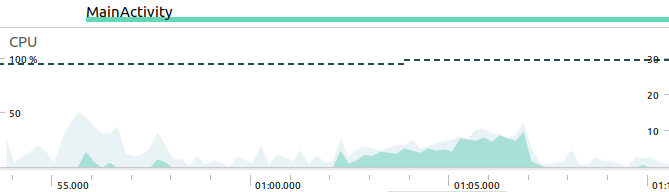
\includegraphics[scale=0.5]{img/cpu.png}
	\caption{Requerimientos de CPU}
	\label{fig:cpu}
\end{figure}

\begin{figure}[H]
\centering
	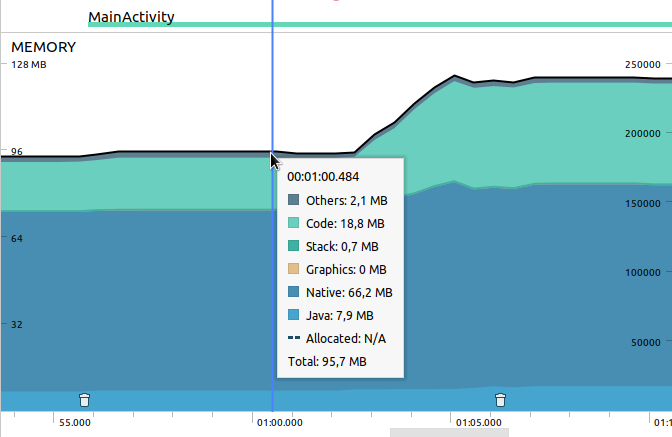
\includegraphics[scale=0.5]{img/memory.png}
	\caption{Requerimientos de memoria}
	\label{fig:memory}
\end{figure}

\section{Mejoras de Android Shield frente a otros trabajos}

Si comparamos este trabajo con otros similares que hemos visto antes, es fácil apreciar que \textit{Android Shield} tiene una precisión superior a todos ellos: 99\% de precisión frente al 85\% de Giang\hypersetup{citecolor=red}\cite{giang}, al 91.8\% de aciertos de Aung\hypersetup{citecolor=red}\cite{aung}, al 93.62\% de precisión de \textit{SIGPID}\hypersetup{citecolor=red}\cite{sigpid} o incluso al que mejores resultados daba, \textit{SFDroid}\hypersetup{citecolor=red}\cite{garg}, con un porcentaje de aciertos del 95.90\%.

Solo Wang\hypersetup{citecolor=red}\cite{cloud} supera la precisión de nuestro trabajo con un 99.71\% de precisión; no obstante, a diferencia de \textit{Android Shield}, Wang lleva a cabo un análisis en la nube, fuera del dispositivo, lo que supone una desventaja.

Por otra parte, \textit{Android Shield} encuentra un punto medio entre el número de permisos utilizados y la precisión alcanzada del modelo. Algunos trabajos utilizan un número muy elevado de permisos para mejorar la precision (como \textit{FDP}\hypersetup{citecolor=red}\cite{jiang}). Analizar un número muy elevado de permisos supone un coste añadido para el dispositivo, que requiere más tiempo de análisis: en este caso tarda alrededor de 15 segundos para analizar 50 aplicaciones.

En el extremo contrario podemos encontrar trabajos que utilizan un conjunto más reducido de permisos. Esto puede ser una ventaja frente a \textit{Android Shield} ya que eliminan ruido que puede confundir al modelo, pero requiere de un preprocesamiento extra, un estudio previo para definir qué permisos son los más útiles para diferenciar entre malware y aplicaciones benignas (como \textit{SIGPID}\hypersetup{citecolor=red}\cite{sigpid}); además, utilizar muy pocos permisos puede afectar a la precisión del modelo como ocurre con Giang\hypersetup{citecolor=red}\cite{giang}.

En cuanto al algoritmo utilizado, hemos comprobado que en \textit{Android Shield} el SVM ha dado unos resultados óptimos, mucho mejores que los demás trabajos. En concreto, \textit{FDP}\hypersetup{citecolor=red}\cite{jiang}, \textit{SIGPID}\hypersetup{citecolor=red}\cite{sigpid} y \hypersetup{citecolor=red}\cite{garg} utilizaban el mismo algoritmo para hacer pruebas, pero, debido a la diferencia de planteamientos, los resultados obtenidos con el algoritmo SVM en estos trabajos no han sido tan buenos como en \textit{Android Shield}. Esto demuestra lo importante que es elegir correctamente las \textit{features} que el modelo va a usar para analizar, pues utilizando el mismo algoritmo los resultados de los tres trabajos mencionados son muy diferentes entre sí, con una clara mejora presentada por \textit{Android Shield}.

Esta comparación se puede ver un poco mejor en la Tabla~\ref{tab:comp-as}.

\begin{table}[H]
\centering
\begin{tabular}{|c|c|c|c|}
\hline
\textbf{Trabajo}        & \textbf{Tipo de análisis}       & \textbf{Algoritmo} & \textbf{Precisión} \\ \hline
\textit{Android Shield} & Estático (on-device)              & PCA + SVM          & 99.11\%               \\ \hline
\hypersetup{citecolor=red}\cite{jiang}                       & Estático (on-device)              & J48                & 94\%               \\ \hline
\hypersetup{citecolor=red}\cite{giang}                       & Estático (on-device)              & Decision tree      & 85\%               \\ \hline
\hypersetup{citecolor=red}\cite{sigpid}                       & Estático (on-device)              & FT                 & 93.62\%            \\ \hline
\hypersetup{citecolor=red}\cite{aung}                       & Estático (on-device)              & K-means clustering & 91.8\%             \\ \hline
\hypersetup{citecolor=red}\cite{cloud}                       & Híbrido (off-device) & SVM + Chi squared  & 99.71\%            \\ \hline
\hypersetup{citecolor=red}\cite{kumar}                       & Estático (on-device) & LSI + Random forest  & 93.92\%            \\ \hline
\hypersetup{citecolor=red}\cite{garg}                       & Estático (on-device) & SVM  & 95.90\%            \\ \hline
\hypersetup{citecolor=red}\cite{todd}                       & Estático (on-device) & Random forest  & 81.53\%            \\ \hline
\end{tabular}
\caption{Comparativa con \textit{Android Shield}}
\label{tab:comp-as}
\end{table}

\section{Tecnologías y bibliotecas utilizadas}

\begin{itemize}
	\item \href{https://developer.android.com/studio}{\textcolor{blue}{AndroidStudio}}: entorno de desarrollo para crear aplicaciones de Android. Cuenta con un emulador de Android (se puede elegir el tipo de dispositivo, la versión de Android...) y una pestaña para que diseñar gráficamente la aplicación sea más cómodo y sencillo.
	\item \href{https://scikit-learn.org/stable/}{\textcolor{blue}{Scikit Learn}}: biblioteca de Machine Learning para Python. Contiene los algoritmos de aprendizaje utilizados (tanto \textit{Naives Bayes} como SVM) así como PCA  y crossvalidation, entre otros.
	\item \href{https://chaquo.com/chaquopy/}{\textcolor{blue}{Chaquopy}}: módulo que permite la integración de Python en aplicaciones Android. Requiere de una licencia, ya sea gratuita para proyectos de código abierto (requiere que el proyecto sea liberado bajo licencia en GitHub o algún otro control de versiones) o de pago para proyectos no libres.
\end{itemize}